% =====================================================================
% Neuromorphic Distributed Hash Table
% David A. Smith, YZ.social
%
% Compile with:  pdflatex nh1-tufte.tex   (run twice for cross-references)
% Requires: tufte-latex, tikz, pgfplots, xcolor
% =====================================================================

\documentclass[nobib]{tufte-handout}

\usepackage[utf8]{inputenc}
\usepackage{tikz}
\usepackage{pgfplots}
\pgfplotsset{compat=1.18}
\usetikzlibrary{positioning, calc}
\usepackage{xcolor}
\usepackage{booktabs}
\usepackage{microtype}
\usepackage{fancyhdr}
\usepackage{etoolbox}
\usepackage{needspace}

% v0.3.48 hotfix: prevent section-heading orphans (heading at the
% bottom of a page with body on the next).  \needspace reserves at
% least 6 baselines of vertical room before each section heading;
% if there isn't that much left on the current page, LaTeX inserts
% a page break before the heading instead of after it.
\pretocmd{\section}{\needspace{6\baselineskip}}{}{}
\pretocmd{\subsection}{\needspace{4\baselineskip}}{}{}

\definecolor{rust}{RGB}{185,78,54}
\definecolor{rustsoft}{RGB}{212,168,150}
\definecolor{inkmuted}{RGB}{102,102,102}

% Roman numeral sections to match the Tufte-book typography
\setcounter{secnumdepth}{1}
\renewcommand{\thesection}{\Roman{section}}

\title{Neuromorphic Distributed Hash Table}
\author[David A. Smith]{David A. Smith \\[0.3em] \emph{\small YZ.social}}
\date{}

\begin{document}

% v0.3.48: tufte-handout's running-header processing applies SOUL
% letterspacing via \MakeTextLowercase, which fails on certain
% page-break points in this document. We use a fancyhdr-based style
% that bypasses the letterspaced running heads but adds visible
% page numbers at the bottom.
\fancypagestyle{ndhtplain}{%
  \fancyhf{}%
  \renewcommand{\headrulewidth}{0pt}%
  \fancyfoot[C]{\thepage}%
}

% --------------------------------------------------------------------
% Custom title page (mirrors the N-DHT whitepaper's half-title)
% --------------------------------------------------------------------
\thispagestyle{empty}
\null\vfill
\begin{center}
{\fontsize{48}{52}\selectfont \textsc{N-DHT}\par}
\vspace{0.6em}
{\Large\itshape Neuromorphic Distributed Hash Table\par}
\vspace{4em}
{\large David A.~Smith\par}
{\itshape\small YZ.social\par}
\vspace{2em}
{\small An N-DHT Explainer \quad v0.3.48 \quad 2026-05-05\par}
\end{center}
\vfill
\null
\newpage

% --------------------------------------------------------------------
% Mission epigraph page
% --------------------------------------------------------------------
\thispagestyle{empty}
\null\vfill
\begin{flushright}
\itshape The technology is shaped by the mission.\par
\end{flushright}
\vfill
\null\newpage

% --------------------------------------------------------------------
% Body opens with page numbers
% --------------------------------------------------------------------
\pagestyle{ndhtplain}
\thispagestyle{ndhtplain}
\setcounter{page}{1}

% --------------------------------------------------------------------
% Hebb body epigraph
% --------------------------------------------------------------------
\begin{quote}
  \itshape Neurons that fire together, wire together.\\[0.3em]
  \normalfont\textsc{\footnotesize Donald Hebb} \,$\cdot$\, 1949
\end{quote}

\vspace{1em}

% =====================================================================
% I. THE MISSION  (copied from N-DHT whitepaper, Chapter 1)
% =====================================================================
\section{The Mission}

\newthought{N-DHT is the engineering substrate} for a privacy-first
decentralized internet. The protocol is designed for a specific job:
to carry the routing and publish/subscribe workload of that internet,
on consumer devices, in real browsers, against the actual physics of
the network it runs on. Everything else about the design---the
architecture, the algorithms, the simulator, the red team, the
deployment path, the application analysis---is shaped by that job.

The job is hard for an unfamiliar reason. The internet of 2026 has
no shortage of clever distributed systems, but almost all of them
are \emph{distributed underneath, central on top}: a constellation
of servers that the user reaches through a single corporate
gateway.\sidenote{The pattern is so common we have stopped noticing
it. CDNs, federated identity providers, cloud auth, app stores, the
``serverless'' frameworks that run on three or four hyperscaler
clouds---all examples of distribution-as-implementation-detail
sitting under a single point of decision.} A real peer-to-peer
internet---one where two strangers can find each other, exchange a
message, and route around an outage without asking permission of any
intermediary---requires a different kind of substrate. The substrate
must be \emph{federation-free at every layer}: addressing, routing,
discovery, group communication, eventual delivery under churn.

\textbf{A distributed hash table is the addressing layer of that
substrate.} Without one, every other peer-to-peer primitive
collapses back into a centralized service: there is no way to find
the user you want to talk to, no way to discover the file you want
to download, no way to subscribe to the channel you want to follow,
without somebody telling you where it lives. With one, those
operations are mechanical: the network itself routes you to the
right peer.

The mission is to build the addressing layer that a real
peer-to-peer internet needs. The protocol described here is what
that addressing layer looks like.

% =====================================================================
% II. THE PROBLEM
% =====================================================================
\section{The Problem}

\newthought{Imagine} you and a million strangers each hold one piece of a giant jigsaw puzzle. Someone walks up and asks for piece~\#438{,}291. How do you find it?

\textbf{Option 1: Have a central directory.} Some company keeps a giant list: ``piece 438{,}291 is held by Alice.'' Easy to look up---but now that company controls everything. They can shut you down, spy on you, charge you money, or just go bankrupt and take the directory with them.

\textbf{Option 2: Give every piece an ``address,'' and design a system where the network \emph{itself} knows how to route requests to the right person, with no central directory.} This is what a \textbf{distributed hash table} (DHT) does.\sidenote{DHTs are the machinery behind BitTorrent, IPFS, parts of Ethereum, and the hidden services on Tor. Every node gets a random ID; every piece of content gets an ID; lookups route from one to the other.}

The trick: how do you find the closest node when you don't know who's in the network and you only know a handful of peers?

The dominant DHT algorithm is called \textbf{Kademlia}, designed in 2002. Every node has a 160-bit ID---a very large random number. To measure ``distance'' between two IDs, you XOR them, comparing bit by bit.\marginnote{\emph{XOR} is a bitwise operation that returns 1 wherever two bits differ and 0 wherever they match. Two IDs that share many leading bits XOR to a small number; two unrelated IDs XOR to a large one.} To find a target, you ask the closest peer you know. They tell you about peers \emph{they} know that are even closer. You ask one of those. Repeat.

The math is clean: each step at least \emph{halves} the remaining distance, so you reach any target in about $\log_2(N)$ hops. With a million nodes, that's 20 steps. Provably correct, used in production all over the internet.

There's just one problem.

% =====================================================================
% III. THE LATENCY TAX
% =====================================================================
\section{The Latency Tax}

\newthought{Twenty hops} sounds fast, but each hop sends a message between two random computers somewhere on Earth. If your peers are scattered randomly across the globe, the average pair sits about half the planet apart---roughly 100~milliseconds round trip.

20 hops $\times$ 100~ms $=$ \textbf{2 seconds.} To find something. Every time.

For real-time applications---voice calls, online games, live messaging, push notifications---2 seconds is unusable. The math says routing is logarithmic, which is fast; the physics says each step is slow because peers are far apart. That's the tension.

The protocol attacks the latency problem with two ideas, one of which is borrowed straight from neuroscience.

% =====================================================================
% IV. G-DHT
% =====================================================================
\section{Putting the Address in the Address}

\newthought{The first idea} is almost embarrassingly simple. It's called \textbf{G-DHT} (Geographic DHT).

Kademlia node IDs are random. A node in Tokyo and a node in Berlin have IDs with no relationship to where they actually are. That's \emph{why} hops are random and slow---random IDs mean random geography.

G-DHT changes one thing: the \textbf{first 8 bits} of every node ID encode where the node says it is on Earth.

The trick uses Google's S2 library, which divides Earth's surface into cells along a curve called a \textbf{Hilbert curve}.\marginnote{Hilbert curves are space-filling: they trace a single continuous path that visits every cell in a grid. Their useful property is that consecutive points on the curve are also adjacent in space.} Its useful property: places near each other on Earth get cell numbers near each other. So XORing two S2 cell numbers gives a small result for nearby places and a large one for distant places.

% --- Figure 1: Hilbert curve --------------------------------------
\begin{figure*}[h]
\centering
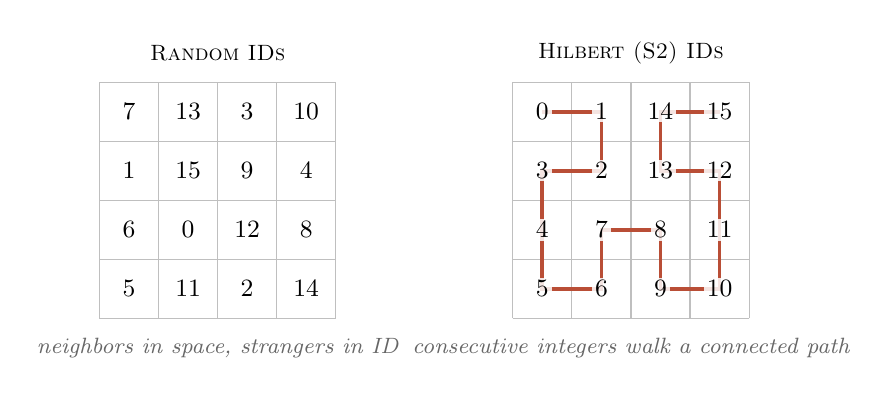
\begin{tikzpicture}[scale=0.75, font=\small]
  % LEFT GRID: Random IDs
  \node[font=\footnotesize\scshape, inner sep=0.5em] at (2, 4.5) {Random IDs};
  \draw[gray!50, thin] (0,0) grid (4,4);
  % numbers
  \foreach \x/\y/\v in {%
    0.5/3.5/7,  1.5/3.5/13, 2.5/3.5/3,  3.5/3.5/10,
    0.5/2.5/1,  1.5/2.5/15, 2.5/2.5/9,  3.5/2.5/4,
    0.5/1.5/6,  1.5/1.5/0,  2.5/1.5/12, 3.5/1.5/8,
    0.5/0.5/5,  1.5/0.5/11, 2.5/0.5/2,  3.5/0.5/14}
    \node at (\x,\y) {\v};
  \node[font=\footnotesize\itshape, color=inkmuted] at (2,-0.5) {neighbors in space, strangers in ID};

  % RIGHT GRID: Hilbert IDs
  \begin{scope}[shift={(7,0)}]
    \node[font=\footnotesize\scshape, inner sep=0.5em] at (2, 4.5) {Hilbert (S2) IDs};
    \draw[gray!50, thin] (0,0) grid (4,4);

    % Hilbert path through cell centers (under numbers, drawn first)
    \draw[rust, line width=1.4pt]
      (0.5,3.5) -- (1.5,3.5) -- (1.5,2.5) -- (0.5,2.5) --
      (0.5,1.5) -- (0.5,0.5) -- (1.5,0.5) -- (1.5,1.5) --
      (2.5,1.5) -- (2.5,0.5) -- (3.5,0.5) -- (3.5,1.5) --
      (3.5,2.5) -- (2.5,2.5) -- (2.5,3.5) -- (3.5,3.5);

    % numbers (over the path)
    \foreach \x/\y/\v in {%
      0.5/3.5/0,  1.5/3.5/1,  2.5/3.5/14, 3.5/3.5/15,
      0.5/2.5/3,  1.5/2.5/2,  2.5/2.5/13, 3.5/2.5/12,
      0.5/1.5/4,  1.5/1.5/7,  2.5/1.5/8,  3.5/1.5/11,
      0.5/0.5/5,  1.5/0.5/6,  2.5/0.5/9,  3.5/0.5/10}
      \node[fill=white, inner sep=1pt, fill opacity=0.85, text opacity=1] at (\x,\y) {\v};
    \node[font=\footnotesize\itshape, color=inkmuted] at (2,-0.5) {consecutive integers walk a connected path};
  \end{scope}
\end{tikzpicture}
\caption[Random vs.\ Hilbert IDs]{Two arrangements of the integers 0--15 on a $4\times4$ grid. With random IDs, sequential numbers scatter unpredictably; cells that are spatial neighbors are numerical strangers. With S2's Hilbert-curve IDs, sequential numbers form a connected path---a continuous walk that never leaves a small neighborhood. XOR distance in ID space now approximates distance on the ground.}
\label{fig:hilbert}
\end{figure*}

Now your node ID looks like: \texttt{[8-bit geographic cell][56-bit hash of public key]}.

The routing algorithm doesn't change at all, but XOR distance now approximately tracks physical distance. When a node looks for a ``close'' peer in ID space, it tends to find one that's also physically close. Local traffic stays local. The 20-hop world tour becomes a 13-hop journey around the neighborhood, with each hop maybe 7~ms instead of 100.

Total: about 91~ms instead of 2~seconds. \textbf{Roughly 20$\times$ faster} for regional traffic, just from changing the \emph{structure} of the addresses.

The cost: nodes can lie about where they are. This is a ``cooperative trust'' assumption.\marginnote{An attacker who falsifies their geographic prefix degrades the locality benefit but not routing correctness. Mitigations exist---learned coordinates, geographic proof-of-work, IP--ASN binding---but G-DHT trades some defense against location-spoofing for a large speedup.} Mitigations exist, but for now G-DHT trades some defense against location-spoofing for a large speedup.

% =====================================================================
% V. NH-1
% =====================================================================
\section{A Network That Learns Like a Brain}

\newthought{The second idea}---neuromorphic routing, which we call \textbf{N-DHT}---is the heart of the protocol. It asks a different question:

\begin{quote}
\itshape What if, instead of engineering shortcuts into the network, the network learned its own shortcuts based on which paths actually work?
\end{quote}

To explain how, we reach for a strange-but-perfect analogy: the human brain.

\subsection{The Engineering Problem That Brains Already Solved}

A single neuron in your brain connects to roughly 10{,}000 others through structures called \textbf{synapses}. There are about 86~billion neurons total. Any given neuron \emph{could} connect to almost any other, but maintaining synapses is energetically expensive---so neurons are stuck with a hard cap, surrounded by far more potential partners than they can afford to keep.

How does the brain decide \emph{which} connections to keep?

This is the same problem facing a peer in a peer-to-peer network. A web browser can only maintain about 50--100 simultaneous WebRTC connections.\marginnote{WebRTC is the technology that lets browsers talk directly to each other, without a server in the middle. Safari caps at about 95 simultaneous connections; Firefox at about 190.} The network might have hundreds of thousands of nodes. Which 50 do you keep?

The brain solved this problem hundreds of millions of years ago. The solution is called \textbf{long-term potentiation}, or LTP.

\subsection{The Brain's Trick}

In 1973, two scientists---Bliss and L\o mo---ran a now-classic experiment. They zapped a particular pathway in a rabbit's brain with high-frequency electrical pulses. Afterward, that pathway responded \emph{more strongly} to subsequent signals---not for seconds, but for \emph{weeks}. The connections had physically gotten stronger.

Decades of follow-up research filled in the details:

\begin{enumerate}
  \item \textbf{The coincidence detector.} Synapses have a special kind of receptor (called NMDA) that only activates when \emph{both} sides of the connection fire at roughly the same time. It's not ``I fired'' or ``you fired''---it's specifically ``we fired together.''
  \item \textbf{The strengthening signal.} When that coincidence happens, calcium rushes in and triggers the synapse to insert \emph{more} of a different kind of receptor (AMPA), making the connection physically more sensitive.
  \item \textbf{Consolidation.} Over the next half hour or so, new proteins get made and new physical structures grow. The change becomes permanent.
  \item \textbf{Decay.} Connections that \emph{don't} get used regularly weaken over time, in a process called long-term depression (LTD).
  \item \textbf{A protective tag.} Recently strengthened synapses get a temporary ``tag'' that protects them from being overwritten by competing changes---but only for a brief window.\marginnote{Without this tag, learning would be self-destructive: the synapses you just learned were useful would be the \emph{first} ones overwritten by the next signal.}
\end{enumerate}

Donald Hebb summarized this in 1949---before the molecular details were known---in the rule that's now bedrock in neuroscience and AI:

\begin{quote}\itshape
Neurons that fire together, wire together.
\end{quote}

Every artificial neural network you've ever heard of---every part of ChatGPT, every image recognition system, every recommendation algorithm---ultimately runs on a digital descendant of this rule.

\subsection{Translating Neurons into Network Routing}

The claim is that the brain's mechanism translates \emph{literally} to peer-to-peer routing---no metaphor needed.

\textbf{NH-1 is the current state-of-the-art N-DHT implementation.}\sidenote{NH-1 is the result of a long sequence of experiments---NX-1 through NX-17---collapsing into twelve rules and twelve parameters governed by a single biology-derived equation. When this document refers to a specific number, it is a number from NH-1. When it refers to the family of neuromorphic routing protocols generically, it says \emph{N-DHT}.} The mapping from neurons to NH-1's routing logic:

\begin{table}[h]
\small
\begin{tabular}{@{}p{0.42\linewidth}p{0.52\linewidth}@{}}
\toprule
\textsc{In the brain\dots} & \textsc{In NH-1\dots} \\
\midrule
A synapse (neural connection) & A connection to a peer \\
Synaptic strength (weight 0 to 1) & A learned weight on each connection \\
LTP: co-firing strengthens & A successful lookup increments the weights along its path \\
LTD: disuse weakens & Every connection slowly decays over time \\
Synaptic tagging (protection) & Recently used connections are protected briefly \\
Pruning of unused connections & Lowest-scoring connection is evicted when a new one wants in \\
\bottomrule
\end{tabular}
\end{table}

That is what NH-1 \emph{is}: a routing system where every connection has a weight that goes up when used and decays when not. The network's ``memory'' is its routing table, and the routing table evolves into whatever shape best serves the actual traffic.

\subsection{The Vitality Function}

The core of NH-1 is a single equation that scores every connection:

\begin{quote}
\centering\itshape
vitality $\;=\;$ weight $\,\times\,$ recency
\end{quote}

The \textbf{weight} is a number between 0 and 1, updated like this:
\begin{itemize}
  \item Every successful lookup that uses the connection raises its weight by 0.05 (capped at 1).
  \item Every ``tick'' of the clock multiplies every weight by 0.995---a slow decay.
\end{itemize}

The \textbf{recency} is 1.0 for the first 20 ticks after a connection is used---the protective tag from synaptic tagging---then drops off exponentially.

% --- Figure 2: Vitality function ----------------------------------
\begin{figure}[h]
\centering
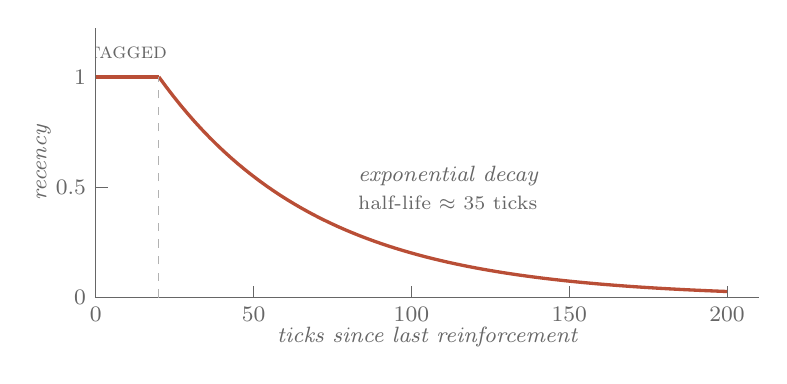
\begin{tikzpicture}[font=\small]
\begin{axis}[
  width=10cm, height=5cm,
  axis lines*=left,
  xlabel={\footnotesize\itshape ticks since last reinforcement},
  ylabel={\footnotesize\itshape recency},
  ylabel style={yshift=-0.5em},
  xlabel style={yshift=0.5em},
  xmin=0, xmax=210,
  ymin=0, ymax=1.22,
  xtick={0,50,100,150,200},
  ytick={0,0.5,1.0},
  yticklabel style={font=\footnotesize, color=inkmuted},
  xticklabel style={font=\footnotesize, color=inkmuted},
  every axis/.append style={color=inkmuted},
  axis line style={color=inkmuted, line width=0.5pt},
  tick style={color=inkmuted}
]
  % flat protected window
  \addplot[domain=0:20, samples=2, line width=1.2pt, color=rust] {1};
  % exponential decay
  \addplot[domain=20:200, samples=80, line width=1.2pt, color=rust]
    {exp(-(x-20)/50)};
  % vertical reference line at t=20
  \draw[gray!60, dashed] (axis cs:20,0) -- (axis cs:20,1);
  % annotations
  \node[font=\footnotesize\scshape, color=inkmuted, anchor=south] at (axis cs:10,1.04) {tagged};
  \node[font=\footnotesize\itshape, anchor=west] at (axis cs:80,0.55) {exponential decay};
  \node[font=\scriptsize, color=inkmuted, anchor=west] at (axis cs:80,0.43) {half-life $\approx$ 35 ticks};
  \node[font=\scriptsize\itshape, color=inkmuted] at (axis cs:20,-0.12) {$t = 20$};
\end{axis}
\end{tikzpicture}
\caption[The recency function]{The recency multiplier in NH-1's vitality function. For 20 ticks after a connection is used, recency stays locked at 1.0---the synaptic tag, protecting freshly learned shortcuts from being immediately overwritten. After that, it decays exponentially with a half-life of about 35 ticks. A connection unused for $\sim$150 ticks contributes essentially nothing to its vitality, regardless of accumulated weight.}
\label{fig:recency}
\end{figure}

When a new connection wants in but the routing table is full, the connection with the lowest vitality gets evicted. Frequently used connections accumulate weight and stay. Unused ones decay and get evicted. Recently strengthened ones are temporarily protected.

That's it. That's the core.

\subsection{Why the Consolidation Matters}

The previous version of this system (called NX-17) had \textbf{18 different rules and 44 parameters} controlling things like ``how full should each part of the routing table be?'' and ``when should we evict a peer?'' and ``how much should we prefer nearby peers?''

NH-1 replaces all of that with the single vitality function plus \textbf{12 rules and 12 parameters}. Letting the connections themselves learn through reinforcement collapses a tangle of rules into one principle.

% =====================================================================
% VI. THE FIVE OPERATIONS
% =====================================================================
\section{The Five Operations}

\newthought{Every behavior} in NH-1 falls into one of five categories---and the categories mirror how \emph{any} adaptive system works:

\textbf{1. Navigate} --- pick the next hop for a lookup. N-DHT scores each candidate by combining XOR distance progress, learned weight, and observed latency. The latency factor halves the score every 100~ms---so a peer that's mathematically a \emph{bit} further but physically a \emph{lot} closer wins.

\textbf{2. Learn} --- strengthen what works. Four mechanisms run on every successful lookup:

\begin{itemize}
  \item \textbf{LTP}: every connection on a \emph{fast} successful path (one that beats the running average of recent path latencies) gets stronger.
  \item \textbf{Hop caching}: every intermediate node along the path remembers the \emph{destination}, not just the next hop. Next time, the path is shorter.
  \item \textbf{Triadic closure}: if you keep seeing peer A relay messages to peer C through you, you introduce them directly. The triangle ``A--you--C'' becomes a direct edge ``A--C.''\marginnote{Named after social network theory: dense triangles emerge in any network shaped by interaction.}
  \item \textbf{Incoming promotion}: peers who keep reaching out to you become candidates for \emph{your} routing table. Passive learning---the network notices who's interested in you, not just who you're interested in.
\end{itemize}

\textbf{3. Forget} --- decay everything that isn't reinforced; evict by vitality.

\textbf{4. Explore} --- inject occasional randomness. A purely greedy router would lock onto the first decent shortcut and never find better ones. N-DHT has two exploration tricks: a ``temperature'' that decays over time but spikes when something breaks (heat up when surprised, cool down when stable), and an ``epsilon-greedy'' rule that picks a random first hop 5\% of the time, just to keep options alive.

\textbf{5. Structure} --- bootstrap and maintain the basic shape of the network when new nodes join.

The template is universal: act, learn from feedback, forget the obsolete, occasionally try something new, maintain basic structure. This is how any good adaptive system has to work.

% =====================================================================
% VII. AXONAL PUB/SUB
% =====================================================================
\section{Axonal Pub/Sub}

\newthought{A real} peer-to-peer network needs more than ``find the node holding key~X.'' It also needs \textbf{broadcast}: a publisher should be able to send a message to all subscribers of a topic, without knowing who they are.

This is publish/subscribe, or ``pub/sub.'' Think of how YouTube notifies subscribers of a new video---except without YouTube being in the middle.

In neuroscience, the \emph{output} of a neuron---the long branching cable that delivers signals to many downstream targets---is called an \textbf{axon}. N-DHT builds axonal delivery trees:

\begin{itemize}
  \item A topic has an ID, derived from the publisher's location and the topic name.
  \item Subscribers send a message routed through the DHT toward that topic ID.
  \item The first node already participating in the topic's tree intercepts the subscriber and adds them as a child.
  \item When a publisher publishes, the message flows from the root down through all the branches.
\end{itemize}

That part is standard. The useful property is that \textbf{the tree heals itself with no special machinery}. Every member of the tree periodically re-issues its subscribe message. If the tree is intact, nothing changes. If a parent died, the re-subscribe naturally lands on whichever live ancestor is now closest. No heartbeats, no failure detection, no parent tracking. The same mechanism that \emph{builds} the tree \emph{repairs} it.

Result: under 5\% churn (5\% of nodes joining and leaving constantly), NH-1 still delivers 100\% of messages. After three refresh cycles, it recovers from any disruption.

% =====================================================================
% VIII. THE THEORETICAL FLOOR
% =====================================================================
\section{Hitting the Theoretical Floor}

\newthought{In 2004}, Frank Dabek and colleagues proved a beautiful, depressing result: \textbf{no recursive DHT can be faster than $3\delta$}, where $\delta$ is the median one-way latency between random pairs of nodes on the Internet.\sidenote{Dabek et al., ``Designing a DHT for low latency and high throughput,'' \emph{Proc.\ NSDI 2004}.}

The proof is geometric. Each hop in a DHT covers half the remaining distance. So the total time is $\delta + \delta/2 + \delta/4 + \delta/8 + \cdots$ which converges to $2\delta$. Add one more hop for final delivery and you get $3\delta$. No matter how clever your routing, no matter how big your network, you can't beat this.

For two decades, no published DHT had been measured at this floor. The best implementations got to maybe $2\times$ the floor.

% --- Figure 3: Dabek floor chart ----------------------------------
\begin{figure*}[h]
\centering
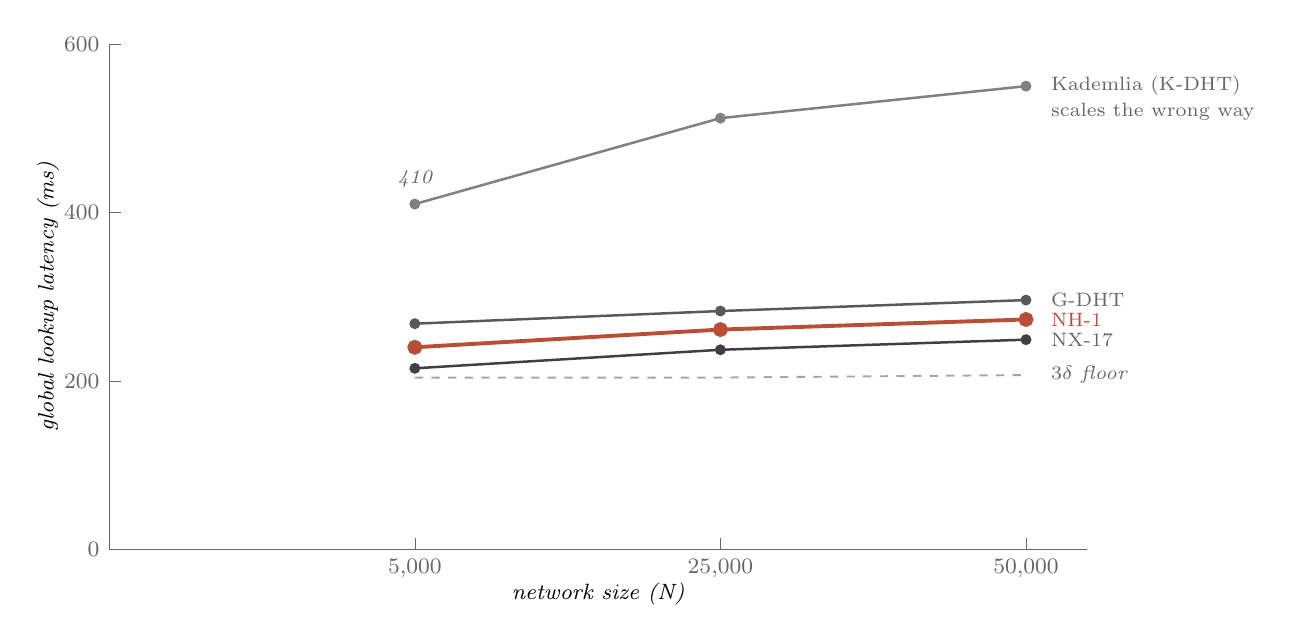
\begin{tikzpicture}[font=\small]
\begin{axis}[
  width=14cm, height=8cm,
  xlabel={\footnotesize\itshape network size (N)},
  ylabel={\footnotesize\itshape global lookup latency (ms)},
  axis lines*=left,
  xmin=0, xmax=3.2,
  ymin=0, ymax=600,
  xtick={1,2,3},
  xticklabels={5{,}000, 25{,}000, 50{,}000},
  ytick={0,200,400,600},
  yticklabel style={font=\footnotesize, color=inkmuted},
  xticklabel style={font=\footnotesize, color=inkmuted},
  axis line style={color=inkmuted, line width=0.5pt},
  tick style={color=inkmuted},
  ylabel style={yshift=-0.5em},
  xlabel style={yshift=0.5em},
  clip=false
]
  % 3 delta floor (dashed reference)
  \addplot[gray!70, dashed, line width=0.7pt] coordinates {(1,204) (2,204) (3,207)};
  \node[font=\scriptsize\itshape, color=inkmuted, anchor=west] at (axis cs:3.05,207) {$3\delta$ floor};

  % K-DHT (light gray, climbs)
  \addplot[gray, line width=0.9pt, mark=*, mark size=1.5pt] coordinates {(1,410) (2,512) (3,550)};
  \node[font=\scriptsize, color=inkmuted, anchor=west] at (axis cs:3.05,550) {Kademlia (K-DHT)};
  \node[font=\scriptsize, color=inkmuted, anchor=west] at (axis cs:3.05,520) {scales the wrong way};
  \node[font=\scriptsize\itshape, color=inkmuted, anchor=south] at (axis cs:1,418) {410};

  % G-DHT
  \addplot[gray!70!black, line width=0.9pt, mark=*, mark size=1.5pt] coordinates {(1,268) (2,283) (3,296)};
  \node[font=\scriptsize, color=inkmuted, anchor=west] at (axis cs:3.05,296) {G-DHT};

  % NH-1 (accent)
  \addplot[rust, line width=1.4pt, mark=*, mark size=2pt] coordinates {(1,240) (2,261) (3,273)};
  \node[font=\scriptsize, color=rust, anchor=west] at (axis cs:3.05,273) {NH-1};

  % NX-17 (dark)
  \addplot[gray!50!black, line width=0.9pt, mark=*, mark size=1.5pt] coordinates {(1,215) (2,237) (3,249)};
  \node[font=\scriptsize, color=inkmuted, anchor=west] at (axis cs:3.05,249) {NX-17};

\end{axis}
\end{tikzpicture}
\caption[Latency vs.\ network size]{Global lookup latency versus network size, plotted against the Dabek $3\delta$ analytical floor (gray dashed). Kademlia \emph{worsens} as the network grows---more hops, each at full pairwise latency, each contributing fully to the total. NX-17 hugs the floor at $1.16\times$; NH-1 at $1.27\times$. The remaining $\sim$20\% overhead matches what the geometric series predicts for 4--5 hops where an ideal protocol takes 3.}
\label{fig:floor}
\end{figure*}

NH-1's predecessor, NX-17, hits \textbf{$1.16\times$ the floor} at 25{,}000 nodes. NH-1 hits \textbf{$1.27\times$}. They sit at the theoretical limit. The remaining $\sim$20\% overhead is structural---they take about 4 to 5 hops where an ideal protocol would take 3, and each ``extra'' hop costs about $\delta/2$, exactly as the geometric series predicts.

For comparison, plain Kademlia \emph{gets worse} as the network grows: $2.01\times$ the floor at 5{,}000 nodes, $2.65\times$ at 50{,}000. It scales the wrong way.

% =====================================================================
% IX. ABLATION
% =====================================================================
\section{Is It the Learning, or the Geography?}

\newthought{A skeptic} would push back: ``Sure, but maybe the geographic prefix is doing all the real work. The brain-inspired learning is gravy.''

An \textbf{ablation study} answers this.\marginnote{An ablation study removes one feature and re-runs everything to see what that feature actually contributed. It's the cleanest way to attribute a result to a specific mechanism.} Strip the geographic prefix entirely---random IDs again---and re-run the comparison.

Result: with \textbf{zero geographic information}, NX-17 still routes \textbf{26\% faster than Kademlia}, and NH-1 routes \textbf{8\% faster}. The learning is doing real work, not sharpening pre-existing geographic structure.

This is the kind of clean control experiment that should accompany any claim of this kind.

% =====================================================================
% X. SLICE WORLD
% =====================================================================
\section{Slice World}

\newthought{The sharpest} demonstration is the \textbf{Slice World} test. The network gets cut almost in half---Eastern hemisphere on one side, Western on the other, connected only through a \emph{single node} near Hawaii. Every other cross-hemisphere connection is severed.

Can the protocol still route messages between hemispheres?

\begin{itemize}
  \item \textbf{Plain Kademlia: 0\% success.} With no learning, the partition is permanent.
  \item \textbf{G-DHT (geography only, no learning): 4.6\% success.} The geographic prefix accidentally points a few peers at the bridge, but nothing builds on the discovery.
  \item \textbf{NX-17 and NH-1: $\sim$94\% success.}
\end{itemize}

% --- Figure 4: Slice World ----------------------------------------
\begin{figure*}[h]
\centering
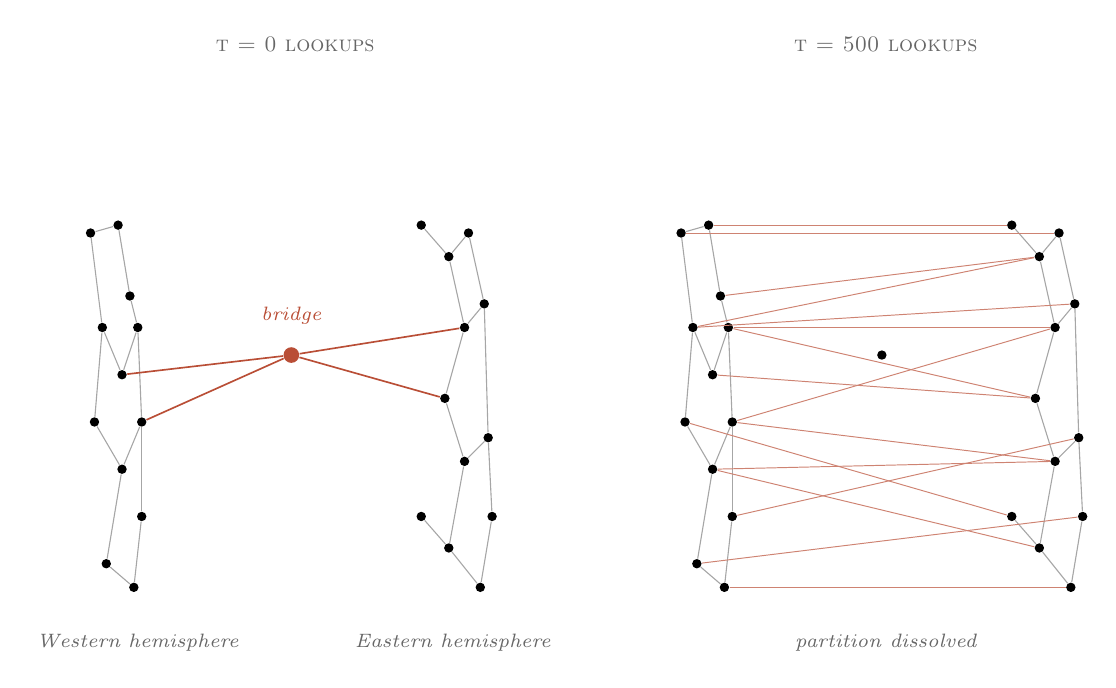
\begin{tikzpicture}[font=\small,
    node distance=0pt,
    dot/.style={circle, fill=black, inner sep=1.2pt},
    bridgedot/.style={circle, fill=rust, inner sep=2pt},
    edge/.style={gray!70, line width=0.4pt},
    bedge/.style={rust, line width=0.6pt},
    cedge/.style={rust!70, line width=0.35pt}
]

% ============ PANEL A: t = 0 ============
\begin{scope}
  \node[font=\footnotesize\scshape, color=inkmuted] at (3.0, 7) {t = 0 lookups};

  % Left cluster nodes
  \node[dot] (LA1)  at (0.4, 4.6)  {};
  \node[dot] (LA2)  at (0.75,4.7)  {};
  \node[dot] (LA3)  at (0.9, 3.8)  {};
  \node[dot] (LA4)  at (0.55,3.4)  {};
  \node[dot] (LA5)  at (0.8, 2.8)  {};
  \node[dot] (LA6)  at (1.0, 3.4)  {};
  \node[dot] (LA7)  at (0.45,2.2)  {};
  \node[dot] (LA8)  at (0.8, 1.6)  {};
  \node[dot] (LA9)  at (1.05,2.2)  {};
  \node[dot] (LA10) at (0.6, 0.4)  {};
  \node[dot] (LA11) at (0.95,0.1)  {};
  \node[dot] (LA12) at (1.05,1.0)  {};

  % Right cluster nodes
  \node[dot] (RA1)  at (4.6, 4.7)  {};
  \node[dot] (RA2)  at (4.95,4.3)  {};
  \node[dot] (RA3)  at (5.2, 4.6)  {};
  \node[dot] (RA4)  at (5.4, 3.7)  {};
  \node[dot] (RA5)  at (5.15,3.4)  {};
  \node[dot] (RA6)  at (4.9, 2.5)  {};
  \node[dot] (RA7)  at (5.15,1.7)  {};
  \node[dot] (RA8)  at (5.45,2.0)  {};
  \node[dot] (RA9)  at (4.6, 1.0)  {};
  \node[dot] (RA10) at (4.95,0.6)  {};
  \node[dot] (RA11) at (5.35,0.1)  {};
  \node[dot] (RA12) at (5.5, 1.0)  {};

  % Bridge
  \node[bridgedot] (BA) at (2.95, 3.05) {};
  \node[font=\scriptsize\itshape, color=rust] at (2.95, 3.55) {bridge};

  % Within-cluster edges (left)
  \draw[edge] (LA1)--(LA2); \draw[edge] (LA2)--(LA3);
  \draw[edge] (LA1)--(LA4); \draw[edge] (LA4)--(LA5);
  \draw[edge] (LA5)--(LA6); \draw[edge] (LA6)--(LA3);
  \draw[edge] (LA4)--(LA7); \draw[edge] (LA7)--(LA8);
  \draw[edge] (LA8)--(LA9); \draw[edge] (LA9)--(LA6);
  \draw[edge] (LA8)--(LA10); \draw[edge] (LA10)--(LA11);
  \draw[edge] (LA11)--(LA12); \draw[edge] (LA12)--(LA9);
  % Within-cluster edges (right)
  \draw[edge] (RA1)--(RA2); \draw[edge] (RA2)--(RA3);
  \draw[edge] (RA3)--(RA4); \draw[edge] (RA4)--(RA5);
  \draw[edge] (RA5)--(RA2); \draw[edge] (RA5)--(RA6);
  \draw[edge] (RA6)--(RA7); \draw[edge] (RA7)--(RA8);
  \draw[edge] (RA8)--(RA4); \draw[edge] (RA7)--(RA10);
  \draw[edge] (RA10)--(RA11); \draw[edge] (RA11)--(RA12);
  \draw[edge] (RA12)--(RA8); \draw[edge] (RA9)--(RA10);

  % Bridge edges
  \draw[bedge] (LA5)--(BA); \draw[bedge] (LA9)--(BA);
  \draw[bedge] (BA)--(RA6); \draw[bedge] (BA)--(RA5);

  \node[font=\scriptsize\itshape, color=inkmuted] at (1.0, -0.6) {Western hemisphere};
  \node[font=\scriptsize\itshape, color=inkmuted] at (5.0, -0.6) {Eastern hemisphere};
\end{scope}

% ============ PANEL B: t = 500 ============
\begin{scope}[shift={(7.5,0)}]
  \node[font=\footnotesize\scshape, color=inkmuted] at (3.0, 7) {t = 500 lookups};

  % Same nodes
  \node[dot] (LB1)  at (0.4, 4.6)  {};
  \node[dot] (LB2)  at (0.75,4.7)  {};
  \node[dot] (LB3)  at (0.9, 3.8)  {};
  \node[dot] (LB4)  at (0.55,3.4)  {};
  \node[dot] (LB5)  at (0.8, 2.8)  {};
  \node[dot] (LB6)  at (1.0, 3.4)  {};
  \node[dot] (LB7)  at (0.45,2.2)  {};
  \node[dot] (LB8)  at (0.8, 1.6)  {};
  \node[dot] (LB9)  at (1.05,2.2)  {};
  \node[dot] (LB10) at (0.6, 0.4)  {};
  \node[dot] (LB11) at (0.95,0.1)  {};
  \node[dot] (LB12) at (1.05,1.0)  {};
  \node[dot] (RB1)  at (4.6, 4.7)  {};
  \node[dot] (RB2)  at (4.95,4.3)  {};
  \node[dot] (RB3)  at (5.2, 4.6)  {};
  \node[dot] (RB4)  at (5.4, 3.7)  {};
  \node[dot] (RB5)  at (5.15,3.4)  {};
  \node[dot] (RB6)  at (4.9, 2.5)  {};
  \node[dot] (RB7)  at (5.15,1.7)  {};
  \node[dot] (RB8)  at (5.45,2.0)  {};
  \node[dot] (RB9)  at (4.6, 1.0)  {};
  \node[dot] (RB10) at (4.95,0.6)  {};
  \node[dot] (RB11) at (5.35,0.1)  {};
  \node[dot] (RB12) at (5.5, 1.0)  {};
  \node[dot] (BB) at (2.95, 3.05) {};

  % Within-cluster edges (same)
  \draw[edge] (LB1)--(LB2); \draw[edge] (LB2)--(LB3);
  \draw[edge] (LB1)--(LB4); \draw[edge] (LB4)--(LB5);
  \draw[edge] (LB5)--(LB6); \draw[edge] (LB6)--(LB3);
  \draw[edge] (LB4)--(LB7); \draw[edge] (LB7)--(LB8);
  \draw[edge] (LB8)--(LB9); \draw[edge] (LB9)--(LB6);
  \draw[edge] (LB8)--(LB10); \draw[edge] (LB10)--(LB11);
  \draw[edge] (LB11)--(LB12); \draw[edge] (LB12)--(LB9);
  \draw[edge] (RB1)--(RB2); \draw[edge] (RB2)--(RB3);
  \draw[edge] (RB3)--(RB4); \draw[edge] (RB4)--(RB5);
  \draw[edge] (RB5)--(RB2); \draw[edge] (RB5)--(RB6);
  \draw[edge] (RB6)--(RB7); \draw[edge] (RB7)--(RB8);
  \draw[edge] (RB8)--(RB4); \draw[edge] (RB7)--(RB10);
  \draw[edge] (RB10)--(RB11); \draw[edge] (RB11)--(RB12);
  \draw[edge] (RB12)--(RB8); \draw[edge] (RB9)--(RB10);

  % Many cross-cluster edges (newly grown shortcuts)
  \draw[cedge] (LB2)--(RB1); \draw[cedge] (LB3)--(RB2);
  \draw[cedge] (LB6)--(RB5); \draw[cedge] (LB5)--(RB6);
  \draw[cedge] (LB9)--(RB7); \draw[cedge] (LB8)--(RB10);
  \draw[cedge] (LB11)--(RB11); \draw[cedge] (LB12)--(RB8);
  \draw[cedge] (LB1)--(RB3); \draw[cedge] (LB4)--(RB4);
  \draw[cedge] (LB7)--(RB9); \draw[cedge] (LB10)--(RB12);
  \draw[cedge] (LB6)--(RB6); \draw[cedge] (LB8)--(RB7);
  \draw[cedge] (LB4)--(RB2); \draw[cedge] (LB9)--(RB5);

  \node[font=\scriptsize\itshape, color=inkmuted] at (3.0, -0.6) {partition dissolved};
\end{scope}

\end{tikzpicture}
\caption[Slice World partition recovery]{At $t=0$ (left), the partition has a single bridge node connecting two hemispheres. By $t=500$ lookups (right), hop caching has installed cross-hemisphere shortcuts in many intermediate nodes; triadic closure has converted observed transit pairs into direct edges. The bridge is no longer special. The protocol does not keep finding the bridge---it uses the bridge to rebuild the bridges that were cut.}
\label{fig:slice}
\end{figure*}

The bridge becomes a \textbf{seed crystal}. After just 10 lookups through the partition, hop caching has installed cross-hemisphere edges in many intermediate nodes. Triadic closure creates direct connections between peers that keep meeting through the bridge. By 500 lookups, hundreds of cross-hemisphere connections exist. The partition has effectively dissolved.

The protocol doesn't keep finding the bridge---it \emph{uses} the bridge to rebuild the bridges that were cut. Like a brain forming new pathways around damaged tissue.

% =====================================================================
% XI. THE HONEST FOOTNOTES
% =====================================================================
\section{What the Simulator Doesn't Model}

\newthought{It is worth} being explicit about what \emph{isn't} measured.

The simulator runs about 25{,}000 lines of JavaScript code modeling the network, but it abstracts away several real-world frictions:

\begin{itemize}
  \item \textbf{Connection setup time.} Real WebRTC connections take 1.5--3~seconds to negotiate. The simulator treats them as instant, so real-world recovery from partitions will be slower than the simulator suggests.
  \item \textbf{Timeout windows.} Real RPCs to dead nodes stall for seconds before failing. The simulator detects death instantly.
  \item \textbf{Bandwidth saturation.} Initially feared as a \emph{success-disaster} failure mode for adaptive routing---that AP scoring's preference for fast peers might funnel traffic onto a few overloaded nodes, oscillating as they collapse and recover. Recent simulations measure the per-node traffic distribution directly and the result is the opposite: at every tested scale ($5{,}000$ to $50{,}000$ nodes), N-DHT distributes load broadly across the population while plain Kademlia and G-DHT concentrate it. At $50{,}000$ nodes, \emph{zero} N-DHT nodes process more than $100\times$ the network mean traffic; K-DHT produces $56$ such nodes, G-DHT produces $62$. Bandwidth concentration is much less of an issue for N-DHT than for K-DHT---not a non-issue, but not the deploy blocker first feared.
  \item \textbf{Latency jitter.} Real round-trip times vary by $\pm$30\% from queuing and congestion. The simulator's latencies are clean and monotone.
\end{itemize}

These get called out in a separate red-team analysis.\sidenote{The companion red-team analysis ranks thirteen deployment-relevant gaps by severity and time-to-fix.} The protocol's measured results show \textbf{the brain working perfectly}; the \emph{body}---actually deploying it on real internet conditions---still needs work.

% =====================================================================
% XII. PLASTICITY OF PLASTICITY
% =====================================================================
\section{Plasticity of Plasticity}

\newthought{The most interesting} future direction is \textbf{metaplasticity}---plasticity of plasticity. In real brains, the rules governing learning \emph{themselves} change based on the brain's activity level. A neuron that's been very active becomes harder to strengthen further (otherwise everything saturates). A neuron that's been quiet becomes easier. The learning rules adapt.

NH-1's parameters---decay rate, protection window, exploration rate---are currently hand-picked constants. A metaplastic version would let the network self-tune them based on local conditions. A peer in a stable region would adapt slowly. A peer in a high-churn region would adapt aggressively. The user would set one knob---``I want my lookup failure rate below 1\%''---and the network would tune itself to hit it.

That's the next layer of brain-inspired self-organization, and the natural endpoint of the path the protocol lays out.

% =====================================================================
% XIII. WHY THIS MATTERS
% =====================================================================
\section{Why This Matters}

\newthought{Step back} from the technical details. The big idea:

\textbf{A peer-to-peer network and a brain face the same engineering problem}---limited connection capacity, vastly more candidates than slots, and the need to figure out which connections are useful.

\textbf{The brain's hundreds-of-millions-of-years-old solution maps directly onto network routing.} Strengthen what works. Decay what doesn't. Protect recent learning briefly so it isn't immediately overwritten. Occasionally explore. The result is a network whose structure is shaped by the traffic it carries, rather than by rules an engineer guessed at.

This isn't just a faster DHT. It's a demonstration that adaptive systems with the right learning rules find their own structure---that decades of brain research can collapse a 44-parameter system into a 12-parameter one, and that you can hit a theoretical limit that's stood for two decades by importing the right idea from a different field.

Code, data, simulator, and the red-team analysis criticizing it are open source.

\end{document}
